\documentclass[]{exam}
\usepackage{amssymb}
\usepackage{amsfonts}
\usepackage{amsmath}
\usepackage{amsthm}
\usepackage[top=1in, bottom=1.5in, left=1in, right=1in]{geometry}
\usepackage{tikz}
\usepackage{pgfplots}
\usepackage{empheq}
\usepackage{mathrsfs}
\checkboxchar{$\Box$}
\usepackage{graphicx}
\usepackage{caption}
\usepackage{float}
\usepackage{enumerate}
\usepackage{comment}
\usepackage{multicol}
\usepackage{color}
\usepackage{advdate}
\usepackage{gensymb}
\usetikzlibrary{arrows}
\usepackage{multirow}
\usepackage{arydshln}
\usepackage{verbatim}

\usepackage{pgfkeys,pgfcalendar}

\newcount\pgfdatecount
\newcommand{\tomorrow}{%
\pgfcalendardatetojulian{\year-\month-\day+1}{\pgfdatecount}
\pgfcalendarjuliantodate{\the\pgfdatecount}{\myyear}{\mymonth}{\myday}
\pgfcalendarmonthname{\mymonth}\space\myday,\space\myyear%
}

\newcommand{\advanceday}[1][1]{
\begingroup
\AdvanceDate[#1]
\today
\endgroup}

\newcommand{\de}[2]{\frac{d #1}{d #2}}


\newcommand{\vertex}{\node[vertex]}
\tikzstyle{vertex}=[circle, draw, inner sep=0pt, minimum size=6pt]
\usepackage{lastpage} 
\usepackage{extramarks}
\usepackage{graphicx} 
\usepackage{tikz}
\usepackage{sectsty} 
\usepackage{amsmath,amsfonts,amsthm} 
\usepackage{wrapfig, blindtext}

% Margins
\topmargin=-0.45in
\evensidemargin=0in
\oddsidemargin=0in
\textwidth=6.5in
\textheight=9.0in
\headsep=0.25in 
\numberwithin{equation}{section}
\linespread{1.1} 
\setlength\parindent{0pt} 
\setlength\answerskip{-.075in}
\setlength\answerlinelength{.5in}
\newcommand{\myitem}{\item[-]}

% HEADER AND FOOTER
\pagestyle{headandfoot}
\runningheadrule
\runningfootrule
\firstpageheader{Kutztown University}{  }{MATH 210}
\firstpageheadrule
\runningheader{P4.HW}{ }{MATH 210}
\firstpagefooter{}{}{} 
\runningfooter{}{}{Page \thepage\ of \numpages}


% TITLE PAGE
\newcommand{\assignmentname}{Phase 4 -- Homework} % Assignment title
\newcommand{\coursetitle}{MATH 210 -- Mathematical Computing and Typesetting}
\newcommand{\duedate}{Due: Friday, May 1 by 11:59 PM on D2L} % Update as needed
\newcommand{\readsections}{\, } % Teacher/lecturer
\newcommand{\semester}{\, }
\title{
\vspace{2in}
\textmd{\textbf{\course:\ \assignmentname}}\\
\normalsize\vspace{0.1in}{\duedate}\\
\vspace{0.1in}\large{\textit{\instructor}}
\vspace{3in}
}
\author{\textbf{Author: \authorname}}
\date{Last Updated: \today}

\pointsinrightmargin
\bracketedpoints



\begin{document}
%%%%%%%%%%%%%%%%%%%%%%%%%%%%%%%%%%%%%%%%%%%%%%%%%%%%%
% COMPILE TITLES AND SUCH
%%%%%%%%%%%%%%%%%%%%%%%%%%%%%%%%%%%%%%%%%%%%%%%%%%%%%
\hspace{1in}\\ \vspace{.15in}


\begin{center}
\normalsize
 \fbox{\fbox{\parbox{5.5in}{
        {\bf Instructions:}  Upload the \texttt{tex} file for this document to your Overleaf project.  All solutions shall be completed on this packet by typing your solution in \LaTeX\, in the space provided.  All solutions should be detailed and should clearly demonstrate the process by which you arrived at the answer.  Submit the compiled \texttt{pdf} file to D2L by 11:59 PM on the due date below.  Submit only a single pdf file of your entire packet.  The question will also ask you to make calculations in Python.  Upload any Python files to the appropriate folder in your GitHub repository.  In this folder, a \texttt{py} file is to be submitted for each problem such that when the \texttt{py} file is executed, the output (as presented in Python) is the solution to the problem. Academic dishonesty will not be tolerated.  }}}
\end{center}

\vspace{.5cm}

\begin{center}
	\Huge\textsc{
	\assignmentname}\\[4pt]
        \Large{\textsc{\coursetitle}\\[10pt]}
        \Large{\textsc{\duedate}\\[8pt]}
        \Large{\textsc{\readsections}\\[8pt]}
\end{center}

\vspace{1cm}

%%%%%%%%%%%%%%%%%%%%%%%%%%%%%%%%%%%%%%
% Uncomment the syntax below when you type up the solutions and type 
% your name.
\begin{center}
	\large{\textsc{\textcolor{red}{Solutions by [YOUR NAME HERE]}}}
\end{center}
\vfill

%%%%%%%%%%%%%%%%%%%%%%%%%%%%%%%%%%%%%%
% Reminders:
%%%%%%%%%%%%%%%%%%%%%%%%%%%%%%%%%%%%%%
Remember to begin each \texttt{py} file with \texttt{import numpy as np} and \verb|import matplotlib.pyplot as plt|.  
For this assignment you will also need \verb|from scipy.integrate import solve_ivp|.

% Blank Page
\clearpage

\begin{questions}
%%%%%%%%%%%%%%%%%%%%%%%%%%%%%%%%%%%%%%
% NUMBER 1 
%%%%%%%%%%%%%%%%%%%%%%%%%%%%%%%%%%%%%%

\question Create a file that computes the numerical solution to the following initial value problem
\[ \de{y}{t} = ky\left(1-\frac{y}{M}\right)\left(\frac{y}{m} - 1\right)\, \qquad y(0) = y_0,\]
for parameter values $k>0$, $m>0$, and $M>0$ and an initial value $y_0$.  Your file should plot the solution to the equation with at least three solutions on the same graph, one with $y_0<m$, $m<y_0<M$, and one with $y_0>M$.  In the space below, include the Python figure with a caption.  In the caption, you must which equilibrium states are attracting and which are repelling.  

\pagebreak


%%%%%%%%%%%%%%%%%%%%%%%%%%%%%%%%%%%%%%
% NUMBER 2
%%%%%%%%%%%%%%%%%%%%%%%%%%%%%%%%%%%%%%
 \item Consider the following system of that describes a predator-prey dynamic: 
\begin{align*}
\de{x}{t} & = Rx - 4x^2 - 3xy\\ 
\de{y}{t} & = -2y + xy \end{align*}
where $R>0$ is a real-valued parameter.  In this model, which population is the prey and which is the predator? Briefly justify your answer.  Determine a value of $R$ that makes both populations coexist.  Plot the vector field with the phase plane solution as well.  Include the two figures below.  Describe in a sentence or two what happens to each population as $t \to \infty$. 


\pagebreak 


%%%%%%%%%%%%%%%%%%%%%%%%%%%%%%%%%%%%%%
% NUMBER 3
%%%%%%%%%%%%%%%%%%%%%%%%%%%%%%%%%%%%%%
\question The following schematic represents a chemical process in which a parent peptide (denoted by $P$) breaks down into four smaller components (denoted by $P_i$ for $i = 1, 2, 3, 4$).  The larger components can also break down into smaller components, where $P_4$ is the smallest component.  Here, assume each ``bin'' is a function of time and measures the concentration of each component in the solution.  
\begin{center}
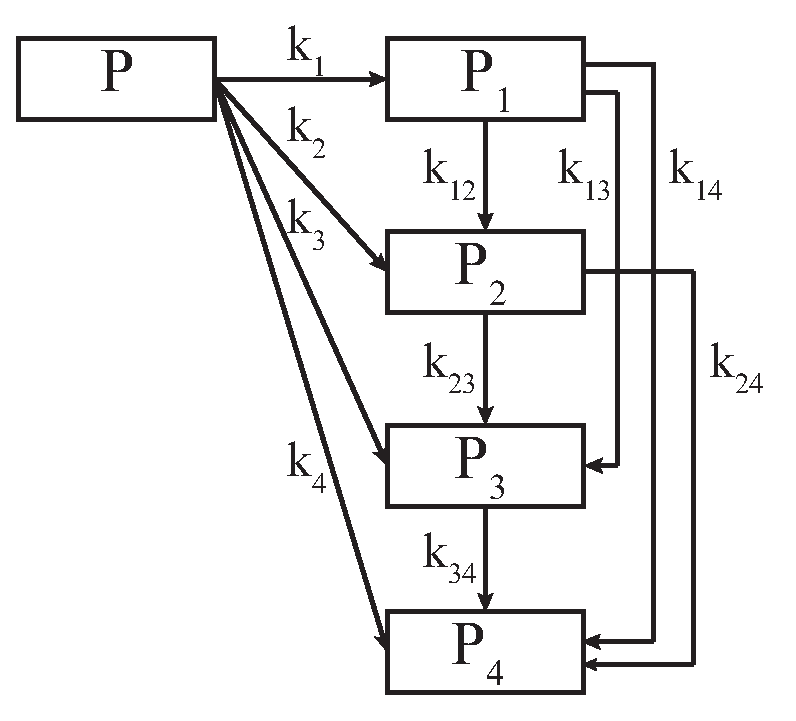
\includegraphics[width = .3\textwidth]{Peptide_Final_Schematic.eps}
\end{center}
Assume that the initial condition contains only the parent peptide, $P(0) = 1$, and all other components are not yet formed: $P_i(0)  = 0$ for $i = 1, 2, 3, 4$.  Set up and write down the linear differential equation model that simulates this process.  Assume each reaction is constant and positive.  Create a file that solves this model and outputs the solution when $k_1 = .09$, $k_2 = .8$, $k_3 = .07$, $k_4 = .6$, $k_{12} = .05$, $k_{13} = .5$, $k_{14} = .06$, $k_{23} = .7$, $k_{24} = .08$, and $k_{34} = .9$.  
Include the figure below in your \LaTeX\, write-up and describe in the caption what happens in this system as $t \to \infty$.  




\end{questions}
\end{document}